\documentclass[12pt,letterpaper]{article}

\usepackage{pslatex}
\usepackage{apacite}
\usepackage{url}
\usepackage{graphicx}
\usepackage{todonotes}

\renewcommand\bibliographytypesize{\small}

\newcommand{\andrew}[1]{\textcolor{magenta}{\bf [#1]}}


\title{Emergent Collective Sensing \\in Human Groups}

\author{
RH or PK --- to be randomized \thanks{MIT Computer Science and Artificial Intelligence Laboratory}
\vspace{-.5em}
\and 
PK or RH --- to be randomized \thanks{Stanford Department of Psychology}
\vspace{-.5em}
\and 
Hongbo Fang (hongbofa@andrew.cmu.edu)\thanks{Department of Computer Science, Carnegie Mellon University}
\vspace{-.5em}
\and
Alex ``Sandy'' Pentland (pentland@mit.edu)\thanks{MIT Media Lab}
\and 
Noah D. Goodman (ngoodman@stanford.edu)$^\dagger$
\and 
Joshua B. Tenenbaum (jbt@mit.edu)$^*$
}

\date{}
\begin{document}

\maketitle
\vspace{-2em}

\begin{abstract}

%Copying successful individuals can be a highly effective way to improve your lot when you're lost in the weeds.


%People are able to copy successful individuals even when success is not readily observable. 

%At the same time, success is not always readily observable.

%While this strategy would seem to be rendered difficult when success is not readily observable, .

%What cognitive abilities enable people to succeed at identifying successful individuals to copy even in such cases when success is obscured or ambiguous.

%Here we argue that flexible agent-reasoning abilities underlie participants' abilities to selectively copy successful individuals in an environment where success can only be inferred from behavior.




%The study of behavioral mechanisms of collective intelligence general regards either rules of thumb or more sophisticated inferential mechanisms that enable 

%Many studies of collective intelligence have documented mechanisms 
%Some have   

%Collective intelligence is the study of 
\todo[inline]{pk: we are confounding literature on small/large populations, as well as literature on collective intelligence versus cultural evolution}
Groups of agents are capable of solving problems that no individual can solve alone. \andrew{Yes, but grouping can also enhance abilities that they already have on their own.  Not sure which is going on here...} 
A variety of simple individual strategies have been proposed to explain such collective intelligence in both humans and non-human animals, such as copying successful individuals or copying when uncertain. 
Yet the cognitive abilities supporting these strategies remain poorly understood.
Here, we propose that social reasoning plays an important role allowing latent properties like ``success'' to be flexibly inferred from outward behavior, such that social learning can be balanced with exploration. 
%While intelligent behavior emerges only at large group sizes for many nonhuman species (e.g. fish or insects), humans rapidly benefit from social interaction even in small teams. 
%In this paper, we take a comparative approach to identify candidate  mechanisms of social cognition that may account for distinctively human forms of collective intelligence. 
%While a variety of simple mechanisms have been proposed to account for 
%Despite its importance, human collective intelligence remains enigmatic.  
%We know what features are predictive of collective intelligence in human groups, but we do not understand the specific mechanisms that lead to the emergence of this distributed information processing ability. 
%In contrast, there is a well-developed literature of experiments that have exposed the mechanisms of collective intelligence in nonhuman animal species.
In Experiment 1, we designed a collective search paradigm for human participants, inspired by the nonhuman animal literature, and found that performance quickly improves as a function of group size. 
%for groups of up to six human participants.
In Experiment 2, we placed human participants in scenarios with artificial agents that were explicitly constructed to evaluate the role of two mechanisms: independent exploration and targeted copying based on social inferences about who is currently successful. 
%We further validated our experimental results by implementing these mechanisms in a computational model: a simulated agent equipped with these mechanisms explained human performance better than models relying on other simple heuristics that have been proposed for nonhuman animals.
Finally, in Experiment 3, we generalize these results to groups in a more complex and noisy environment.
Taken together, we find that even the most rudimentary mechanisms of human social cognition affords robust and flexible use of social learning strategies. \todo[inline]{pk: i find the phrase cognitive mechanisms and similar quite confusing in the context of this paper. i think we are studying behavioral mechanisms and cognitive abilities.}

\textbf{Keywords:}
  collective intelligence; distributed cognition;
  social cognition; social computation; online experiments
\end{abstract}

\section{Introduction}

%Social learning enable culture. allows things to be cumulative. it's important!

%Learn to preferentially copy successful individuals even when success must be inferred.

%in the animal literature, socila learning mechanisms have mostly bee studied as these strategies

%here are vatrious mechanisms tha thave been proposed
%these mechanismstic account have succesfully provided finew-groaunded analysical, explained collecitv ebavhior in a lot of caase. these stratgeies also cna mostly be explained by through behavioral associative learning (andrew social foraging ref)

%in parallel to all this, there has been a bunch of social cognition work about the way people make inference. there has bene a lot of work in social learning in cogsci, but mostly isn;t used ot explain big emergenyt things. mostly local


%tehre has been stuff about cognitive abilities predicting ermgey things, but this is generally about measuring things about individual that you can predict things tfrom rather than interactive mechanisms.


%in the present work, we aim ot ground the emergeny thing in the more immedaiate, cognitively orienteg mechanisms.

%in the cases where models are used in human collective intelligence, the models tend to be the same as animal behavior litearutre, in that reward is modeled as visible. not so much social inferece mechanisms. 


%meanwhile the cognitve sciene litatrure,a whic has also been interested in social learnk ,has tended ot think of things less as sttrategyie sand more as cognitive abilitesy---inferences that agents can make, theory of mind 

%gap: what if the actual reward is hidden. then what?

%all this social inference stuff is about latent properties of 

%infering prferences, goal, beliefs and desires. things you can't just read off someone's face

%look at a social foraging like task

%but without being able to actually observe what the rewards are there

%copy the successful. it's just so obvious! what if you don't know who is successful

%we know copy successful, but what happens when you don't have direct access to success. 

%its unknow how distirbuted searhc might work in humans where there is potential for more soiphisticated individual mechanisms. 

%what are the two or three main reuslts?

%people can do collective searhc, increas in gropu size

%use agent reasoning

%uniquely suited to this 

%associatve 


\begin{quote}``A boat; hey, I've seen a boat! It passed by now two moments ago. It went...uh, this way; it went this way! Follow me!''\\
-Dory in \textit{Finding Nemo}
\end{quote}

Relying on others can be risky or rewarding. Advice seekers must balance collecting wisdom with getting pulled in different directions, and disentangling good advice from bad. %Getting a sense for who knows what is crucial. 
A group who all know who knows what can be quite effective at solving problems together, but getting that meta-knowledge is not automatic. What abilities enable such achievements of collective intelligence?


%Yet figuring out whose lead to follow requires getting a sense for who knows

%What enables people to 





%Yet discovering this information without explicit instructions requires making inferences from . 

 

%While much work from evolutionary biologists has focused on heuristic descriptions of behavioral rules used in social learning, recent work by cognitive scientists has turned towards understanding the meta-cognitive reasoning and cognitive abilities at play in human social learning. Rather than just studying where, when, and how social observation is employed in decision-making, these cognitive scientists have been interested in understanding the underlying domain-general mental representations people have at their disposal that enable these kinds of social learning in the first place. 

% Paragraph 1 topic sentence: collective intelligence is important and depends on 'social learning'
%From ant colonies to basketball teams, groups of agents are able to accomplish feats of intelligence beyond the reach of any individual.
%Groups are not only able to distribute complex computations across agents more effectively \cite{hutchins_cognition_1995} --- new emergent processes arise from interactions between agents. 
%When agents can observe and learn from one another, they no longer need to independently obtain all of their information from direct experience with the world. 
%Social learning thus allows the group as a whole to cumulatively build on individual successes, and is considered to be a key process driving collective intelligence \cite{boyd2011cultural,tomasello_natural_2014, laland2017darwin}. 
%\todo[inline]{jumping into details (need model paper...?). don't bury the RQ}

% Paragraph 2 topic sentence: social learning needs to be *selective* to be effective, and when/who heuristics are one way of achieving selectivity.
\todo[inline]{rdh: given space constraints, I think this point can be condensed into previous or following paragraph?}
The study of social learning examines how people and other animals make use of information from others around them.
A large body of work in human and non-human animals has focused on what strategies, or heuristics, allow social learning to be effective \cite{laland_social_2004,hoppitt2013social,RendellFogarty___Laland11_CognitiveCulture}. 
Indiscriminate copying, for example, is not an effective strategy. 
As more individuals rely on imitation, rather than independent asocial learning, it becomes increasingly likely that a random target of copying is using outdated or inaccurate information, decreasing the mean performance of the group \cite{rogers_does_1988}.
For the group to benefit from social learning, it must be deployed selectively \cite{kameda2003does,boyd1995does,kendal2005trade}, both in choosing the appropriate time to learn from others (\emph{when} strategies) and choosing the appropriate individuals to learn from (\emph{who} strategies). 
For example, a ``copy-when-uncertain'' heuristic allows an agent to deploy social learning only when independent exploration becomes challenging, or a ``copy-successful-individuals'' heuristic allows an agent to filter out low-quality social information and target other agents most likely to increase their own fitness.

% Paragraph 3 topic sentence: to explain flexibility of human groups, however, we need to go deeper than bundles of heuristics to understand the underlying cognitive mechanisms (e.g. social inference)
Attention has increasingly turned from documenting evidence for individual heuristics to investigating the mechanisms underlying the flexible use of different strategies \cite{heyes2016blackboxing,kendal2018social}. 
Agents often use hybrid strategies, combining multiple sources of \emph{who} or \emph{when} information, or deploy different strategies in different contexts \cite{mcelreath_beyond_2008}.
Thus, it may be useful to view social learning behavior not as the application of an inventory of simple copying rules, but as arising from deeper cognitive mechanisms.
Especially in the case of humans, and some non-human primates, there has been substantial interest in the extent to which social learning relies on mechanisms like meta-cognition \cite{heyes2016knows} or theory of mind \cite{shafto2012learning} that go beyond pure associative learning \cite{behrens2008associative,heyes_whats_2012,heyes2012simple}.
These proposed mechanisms allow agents to maintain explicit representations of ``who knows'' and thus concentrate social learning on particularly knowledgeable individuals.
Similar cognitive mechanisms have been implicated in organization science as predictors of collective intelligence in small groups \cite{woolley2010evidence,engel2014reading}.

% Paragraph 4 topic sentence: these social inference mechanisms may be particularly important for understanding how we flexibly decide who to learn from in environments where we can't directly access others' rewards (i.e. pointing out unrealistic assumption of a lot of previous work in groups, where it's no wonder they were able to get away with simpler heuristics; copying the most successful is easy if there's a button you can press saying exactly how successful everyone is!)
We suggest that these social inference mechanisms may also help shed light on a puzzle raised by \emph{who} heuristics like ``copy-successful-individuals.''
Computational simulations \cite{schlag1998imitate,lazer2007network,rendell_why_2010} and human experiments \cite{mason2008propagation,mesoudi2008experimental,mason2012collaborative} typically provide agents the ability to directly observe the underlying payoffs of different agents (sometimes at a cost).
However, many real-world environments do not provide such direct access. 
Indeed, hiding payoffs can reverse the benefits of selective copying because the solutions of different agents cannot be compared \cite{wisdom_social_2013}.
Accounts of selective copying that rely information about who is successful or knowledgeable must also provide an account of how agents \emph{come to know} this information.
While it is possible that associative learning allows agents to adopt particular external cues as proxies (e.g. visible health or wealth), social inference mechanisms may provide a more flexible alternative. 
Humans continually move between different contexts where success manifests in different observable behaviors: a reliable cue of success in one environment may not be reliable in another.
By inverting a generative model of behavior \cite<e.g.>{jara2016naive,baker2017rational}, agents can make context-sensitive predictions and flexibly infer the hidden success or knowledge of others.

% Paragraph 5 topic sentence: in fact, recent cognitive science has extensively worked out how these mechanisms work in *individual* social learning experiments, but implications for groups & collective intelligence remain unclear
This ability has been extensively studied in cognitive science.
Even young children are able to rapidly infer which partners are more trustworthy and knowledgeable than others, and prefer to learn from them \cite{wood2013whom,sobel2013knowledge,gweon2014sins,poulin2016developmental,harris2018cognitive,mills2016learning}, and adults can appropriately discount unreliable social information in their decision-making \cite{hawthorne2019reasoning,velez2019integrating,WhalenEtAl18_SensitivityToSharedInfo}.
However, this cognitive science literature has largely developed independently from work on social learning strategies in larger collectives.
Previous work in animals has suggested that inferences about underlying cues may prevent costly and erroneous cascades of behavior \cite{bikhchandani1998learning,giraldeau2002potential}, but the broader implications of social inference abilities for collective intelligence remain unclear.

% Paragraph 6 topic sentence: in this paper, we investigate the implications of these social inference mechanisms for groups of humans (i.e. summary of contributions).
In the present work we bridge these two literatures by examining the behavior of human groups in a collective sensing task\footnote{Collective sensing is related to collective foraging tasks \cite{dechaume2005hidden,goldstone2005knowledge}, but the ‘resource’ is not consumable so there are no competitive dynamic.} where others' payoffs are not directly observable.  
This task builds on a recent task designed to study the collective sensing of fish schools  \cite{berdahl_emergent_2013}.
In our experiments, human participants controlled avatars in a virtual world.
Each location corresponded to a hidden score value that fluctuated over time.
They could continually observe the movements of other agents but only had access to the score at their own current location. 
Across three experiments, we used this virtual environment to investigate how the performance of groups changed as a function of group size (Experiment 1), evaluate the individual social learning mechanisms driving collective success (Experiment 2), and measure the effect of noise on social learning (Experiment 3).
%We find that participants were able to preferentially copy agents who are in higher-scoring regions based solely on observable behavioral signatures of `exploiting', even as these signatures differed across experiments.
%Furthermore, during times when no agents in the group were displaying these behaviors, we found that participants preferred to independently explore the environment rather than indiscriminately copy.
Taken together, this work suggests that even in novel environments where the payoff information of other agents is not directly accessible, individual social cognition may nonetheless enable flexible collective intelligence. 

%\section{Related Work}
%\todo{I've put this here for now. Could incorporate into intro instead, or move to discussion, or keep here.}
%\todo[inline]{paragraph 2-3: start by reviewing proposals about the heuristics that might support nonhuman animal CI. then at end, ask if these are sufficient to explain human behavior also. Cecelia Heyes's (2016, 2018) proposal that the ability to explicitly represent ``who knows'' is distinctively human. Also: ``Evidence shows that group size is critical for CTC in that the presence of a high number of models is beneficial for the stability of a trait as well as for innovation through the combination of solutions produced by the different models (Derex & Boyd 2015; Derex et al. 2013a; Kemp & Mesoudi 2014; Muthukrishna et al. 2014). Other evidence has been reported, highlighting an absence of or even an inverse relationship between population size and cumulative performance (Caldwell & Millen 2010; Collard et al. 2005; 2016; Fay et al. 2019; Vaesen et al. 2016).'' }
%Many mathematical and computational of models collective behavior have been proposed to explain the cumulative `ratchet' of human culture, placing the locus of the difference on language (cite), joint coordination (cite), social learning (cite), or technical reasoning (cite). 
%% flocking behavior, collective
%% decision-making, and other simple collective behaviors have been
%% proposed based on coarse observations, scientific intuitions, and
%% informal analogies.
%However, as a result of the logistical difficulties in conducting
%real-time human experiments involving multiple participants, and as a
%result of a broader lack of data analysis aimed at understanding
% collective behavior, the quantitative study of collective behavior has
% largely lacked an empirical basis.  Recently, researchers have begun
% conducting carefully controlled laboratory experiments to test and
% refine models of collective behavior \cite{couzin_collective_2009}.  
% Yet many of these experiments, with
% some notable exceptions \cite{goldstone_collective_2008,
%   kearns_experiments_2012}, have been conducted using nonhuman animal subjects.  %% The logistical
%% difficulties
%% of having multiple human participants simultaneously interacting in a
%% real-time environment are still widely regarded as prohibitive.
% We are therefore quickly developing a better understanding of the
% collective behavior of ants \cite{pratt_tunable_2006}, bees
% \cite{seeley_group_1999}, cockroaches \cite{ame_collegial_2006}, and
% fish \cite{ward_quorum_2008}, but our empirically-grounded
% quantitative understanding of human collective behavior remains
% limited.

%% Furthermore, given that humans are thought to have fundamentally
%% different cognitive abilities than other animals, there is little
%% reason to believe that the models of collective behavior that have
%% been developed for other animals would be appropriate for humans.
%% Our
%% goal is to understand in what ways human performance differs from that
%% of nonhuman animals.
%uniquely human attributes may lead to different outcomes




\section{Experiment 1: Collective sensing across group sizes}

\subsection{Participants}
We recruited 781 unique participants from Amazon Mechanical Turk to participate in this experiment.  All participants were from the United States.  After excluding 52 participants due to inactivity or latency, and 9 others for disconnecting in the first half of the game, we were left with usable data from 720 participants in 312 groups.  These groups ranged in size from one to six individuals. 

\subsection{Stimuli}

\begin{figure}[t!]
  \centering
  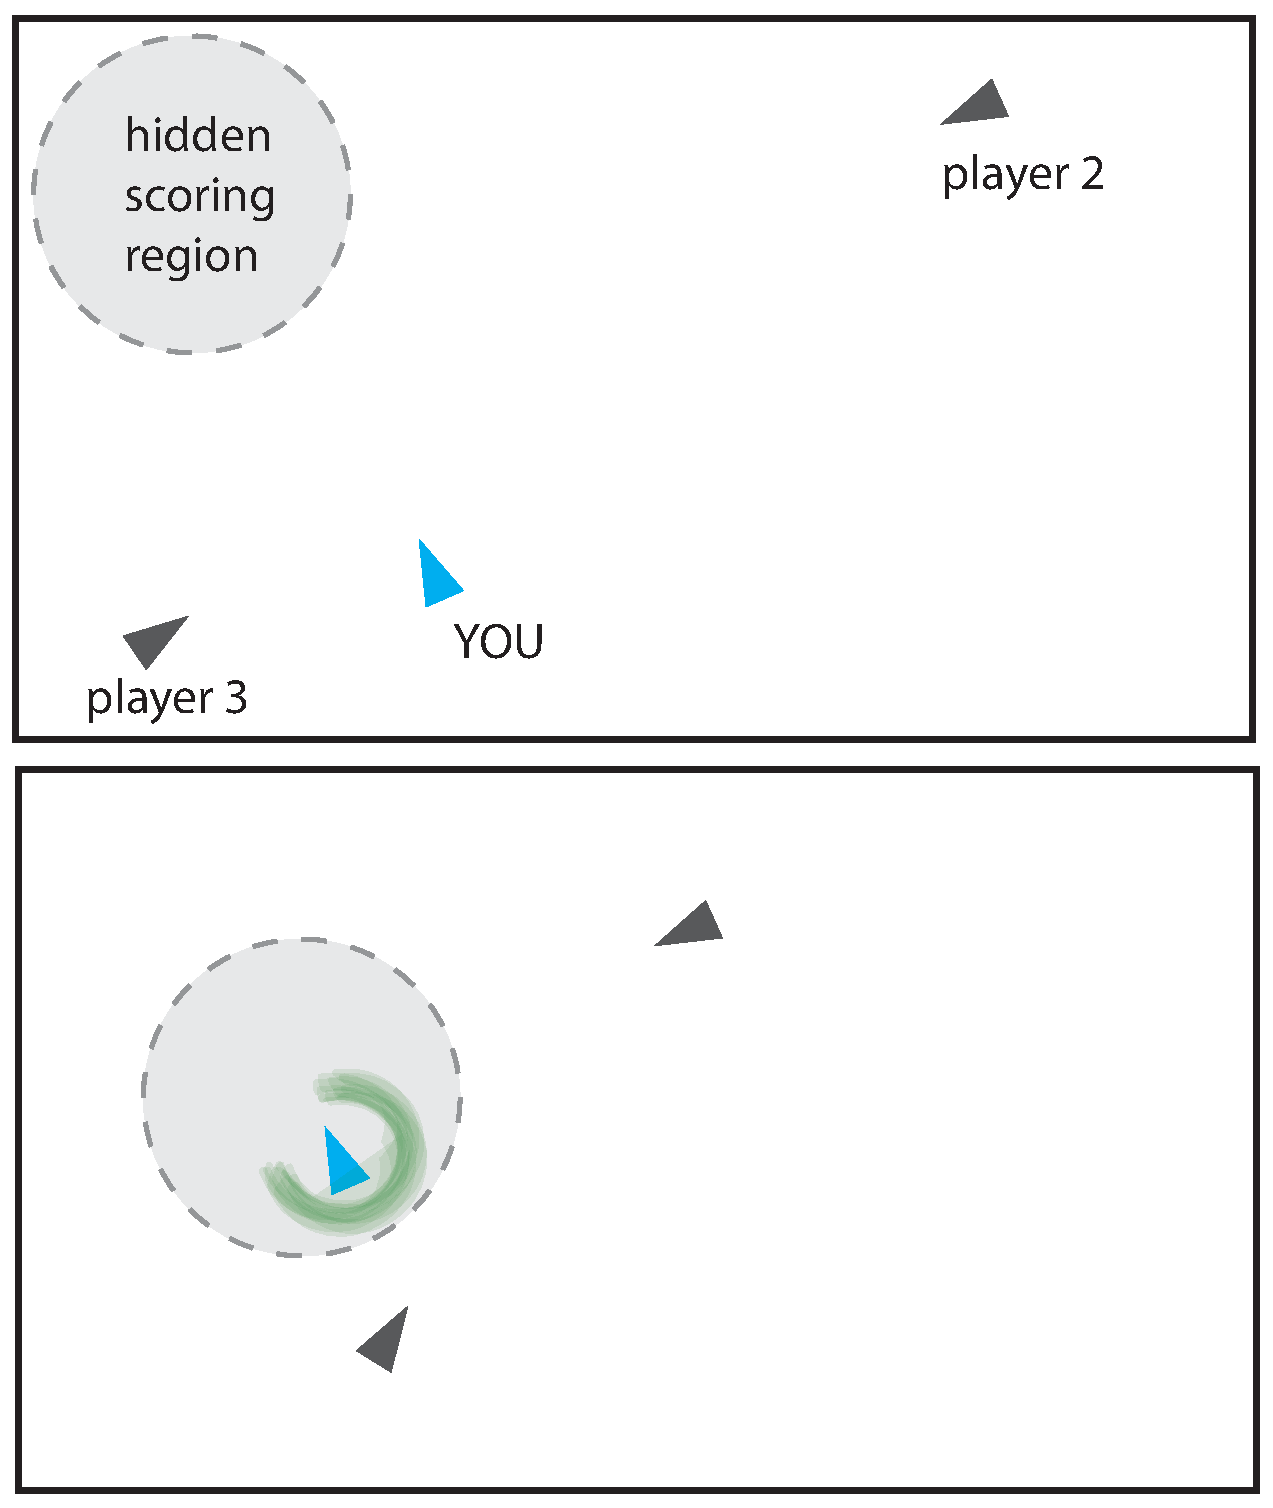
\includegraphics[width=0.6\textwidth]{./figures/experiment1_design.pdf}
  \hspace{0.1cm}
  \caption{Example states of the multi-agent tracking task used in Exp. 1. Hidden scoring region is shown in grey, slowly drifting over time. Bottom frame shows participant receiving a bonus reward upon entering the region. The halo indicating this bonus was only visible to the player inside the region, and not to the other players.}
  \label{fig:score}
\end{figure}

The virtual game environment measured 480 pixels in width and 285 pixels in height.
Avatars were represented by triangles that were 10 pixels in length and 5 pixels in width, rotated to the direction the avatar is facing. 
Players controlled their avatars by clicking and using two keyboard keys. 
Clicking within the playing area instantly oriented the direction of the avatar to be facing the location clicked. 
Participants could hold the ``a" key to accelerate or hold down the ``s" key to stop.  
The avatars automatically moved forward at a constant velocity of 17 pixels per second if no buttons were pressed, but instantaneously increased to a constant velocity of 57 pixels per second for the duration of time that the ``a" key was held down and decreased to 0 pixels per second for the duration of time the "s" key was held down. 

We designed the environment as a multi-agent tracking task (Fig. \ref{fig:score}).
The score that agents obtained at each location at each point in time was determined by an underlying ``score field.'' 
This field was hidden from participants, who only had access to the score at their current location. 
We generated score fields by first initializing a circular region with a diameter of 50 pixels at a random location on the playing area. 
Inside this region, the score was set to 1.
Outside this region, the score was set to 0.
We then moved this region along a straight line to a randomly chosen target location within the playing area at a speed of 17 pixels per second.
Once it reached this location, we selected another target location, and repeated the process for the duration of the experiment.
We pre-generated 5 such score fields, so multiple groups were randomly assigned to the same underlying field.  

Because these simple score fields were binary (i.e. either inside or outside the circular scoring region), we showed participants binary feedback about their current score.
When an avatar entered the circular region, it was surrounded by a salient sparkling halo and the border of the playing area turned green (see supplementary Fig. \ref{fig:supplemental_interface} for screenshots). 
Critically, this feedback was only visible to the participant controlling that avatar; participants did \emph{not} directly observe whether other players were in the scoring region. \andrew{However, participants could see the location and orientation of other participants.}

Each participant played in a single
continuous game lasting for 5 minutes, and locations were updated every 125 milliseconds. 
To discourage inactivity, participants also received 2/3 of a point for each second they were actively participating in the game.
For any moment when an avatar was touching a wall, we displayed a large warning message and set the player's current score to zero so that they stopped accumulating points.

\subsection{Procedure}

After agreeing to participate in our experiment, participants were presented with a set of instructions describing the mechanics of the game, using a cover story framing the game as a search for the ``magical bonus region".  
The participants were informed about the dynamics of the underlying score field and also explicitly informed that ``There is no competition between players; the magical region is not consumed by players. It simply changes location over time." 
Participants were not explicitly instructed or suggested to cooperate or coordinate with each other.

After successfully completing a comprehension test, participants were then redirected to a waiting room.
For each waiting room we started, we randomly sampled a target group size between 1 and 6.
Participants would wait for up to 5 minutes or until the pre-assigned number of other players joined.
While in the waiting room, participants could familiarize themselves with the controls of the game.  Players were not shown any score in
the waiting room unless the participant was against a wall, in which
case the border of the playing region would turn red and a warning appeared on screen.  All players spent at least one minute in the waiting room to help ensure familiarity with the controls before starting the game. 

Both in the waiting room and the actual game, players were removed for inactivity if we detected that they had switched to another browser tab for more than 30 seconds total throughout the game or if the player's avatar was moving into a wall for 30 consecutive seconds.  
We also removed players if their ping response latencies were greater than 125ms for more than 75 seconds in total throughout the game.  
To minimize disruption of large groups, we allowed multi-player games to continue after a participant disconnected or was removed, as long as at one or more participants remained.

We paid participants 75 cents for completing our instructions and comprehension checks, and the participants could receive a bonus of up to \$1.25 during the five minutes of gameplay. Each point in the game corresponded to \$0.01 of bonus. Each participant was also paid 15 cents per minute for any time spent in the waiting room, minus any time that player spent moving into a wall.  These numbers were chosen so that the participants were expected to receive at least a wage of \$9 per hour for the totality of their time active in the
experiment.

We implemented this experiment using the MWERT framework \cite{hawkins_conducting_2014}, which uses a stack of recent web technologies capable of handling the challenges of real-time, multi-player web experiments, including Node.js, the Socket.io module, and HTML5 canvases.  

\begin{figure}[t!]
  \centering
  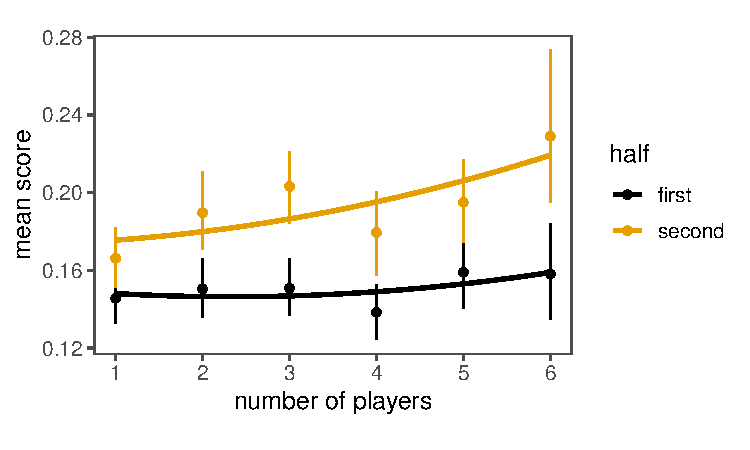
\includegraphics[width=0.8\textwidth]{./figures/performance-summary-exp1.pdf}
  \caption{Mean performance of human participants in each half of Experiment 1 as a function of group size. Larger groups saw significant gains in performance. Error bars are 95\% bootstrap confidence intervals using the group as the primary bootstrap unit. \andrew{Ok, so going back to my other comment (sensing vs learning), this suggests the collective sensing is learned. Is that new/cool/unique, or am I just tired?} }
  \label{fig:exp1_performance}
\end{figure}

\subsection{Results}

We hypothesized that individuals in larger groups would be able to achieve higher scores on average than individuals in smaller groups. 
We also hypothesized that the advantages of larger groups would accrue later in the game, when participants had adjusted to the mechanics of the environment and the behavior of the other players.
To test these hypothesis, we examined performance during each half of the 5-minute session. 
In cases where one or more players were disconnected or removed, we measured the size of the group at the end of the session.
We constructed a mixed-effects regression predicting each individual participant's average score over the time period, including fixed effects of period (first vs. second half), the continuous number of players in their environment (one through six), and their interaction.
We also included random intercepts for each group and each of the five underlying score fields.
First, we found a main effect of practice: scores were significantly higher on the second half of the session ($b = 2.1,t=-10.8, p < 0.001$).
However, we also found a significant interaction with group size: while performance on the first half was similar across group sizes, the performance of each individual on the second half significantly increased in larger group sizes from a score of 0.16 in groups of 1 to 0.24 in groups of 6 ($b = 0.33$, $t = 2.8$, $p = 0.004$; see Fig. \ref{fig:exp1_performance}). 

\section{Experiment 2: Evaluating copying strategies}

What cognitive mechanisms allowed humans in Experiment 1 to benefit from collective intelligence even when the payoff information of other agents is not directly accessible?
We hypothesized that human behavior in this environment is driven by two underlying strategies: (1) independent exploration and (2) precise, targeted copying based on social inferences about success. 
These hypothesized strategies rely on cognitive mechanisms allowing humans to infer ``who knows'' about high-scoring locations based on outward behavioral traces (e.g. slowing down or stopping in a region) and also to inhibit social influence to act independently when appropriate.

The design of Experiment 1 made it challenging to disentangle these strategies.
For example, we were interested in analyzing participant clicks to detect signatures of selective copying, but because there was a unique `spotlight' at each point in time, different copying strategies were confounded: players who were already obtaining reward and trying to stay inside the spotlight were, by necessity, clicking close to other players who were obtaining reward, even if they were not intentionally copying them.

For our second set of experiments, then, we designed a sequence of controlled scenarios that are more diagnostic for testing the use of these different strategies.
We placed participants into an environment with artificial agents that we designed, rather than other humans, and we manipulated the location of the score field to estimate the probability of copying different agents under different conditions.

For conceptual clarity about our design and analysis, it is helpful to define three broad `states': exploring, exploiting, and copying \cite<e.g.>{rendell_why_2010}.
We define \emph{exploiting} as selecting an action that maximizes the expected score given the agent's current knowledge of the environment, i.e. staying close to a known location of the spotlight. 
We define \emph{copying} as forward motion, sometimes accelerated, toward the location of another agent. 
We define \emph{exploring} as selecting an action that has an unknown outcome, often moving to a region without other agents. 
In this environment, exploiting, exploring, and copying behavior were associated with distinct and recognizable movements.
Our hypothesized strategies can be operationalized as selective deployment of these three states: exploiting rather than copying or exploring when one is in a high-scoring region, and copying rather than exploring in low-scoring regions only when it can be inferred that another agent is receiving a high score, based on outward behavioral signatures.

\subsection{Methods}
\subsubsection{Participants}

We recruited 28 unique participants from Amazon Mechanical Turk.
All participants were from the United States.

\subsubsection{Stimuli \& procedure.}

As in our first experiment, participants were given control of an avatar to explore a virtual environment and were rewarded based on their location according to a hidden ``score field.'' 
The interface and controls were the same as in Experiment 1, but the procedure differed in several ways. 
Instead of a single 5-minute session, we designed a sequence of shorter scenarios that were informative for distinguishing between several different potential mechanisms that could be used in the game. Our key experimental manipulations that we used to distinguish between behavioral mechanisms people were employing in this game involved carefully controlling aspects of the score field dynamics and bot behaviors. 

In the environment of Experiment 2, the clearest exploiting behavior is pressing the ``s" button to stop the player avatar, although exploiting can also look like moving slowly or otherwise meandering around near a single location or in a single direction.  The bots we programmed to have more control in Experiment 2 all exploit by stopping.  We operationalize copying behavior simply as moving towards another agent.  Exploring behavior in Experiment 2 encompasses all other kinds of behavior displayed.
The experiment was structured into a sequence of two phases: a \emph{practice} phase and an \emph{test} phase (see Fig. \ref{fig:exp2_design}A).

\begin{figure}[t!]
  \centering
  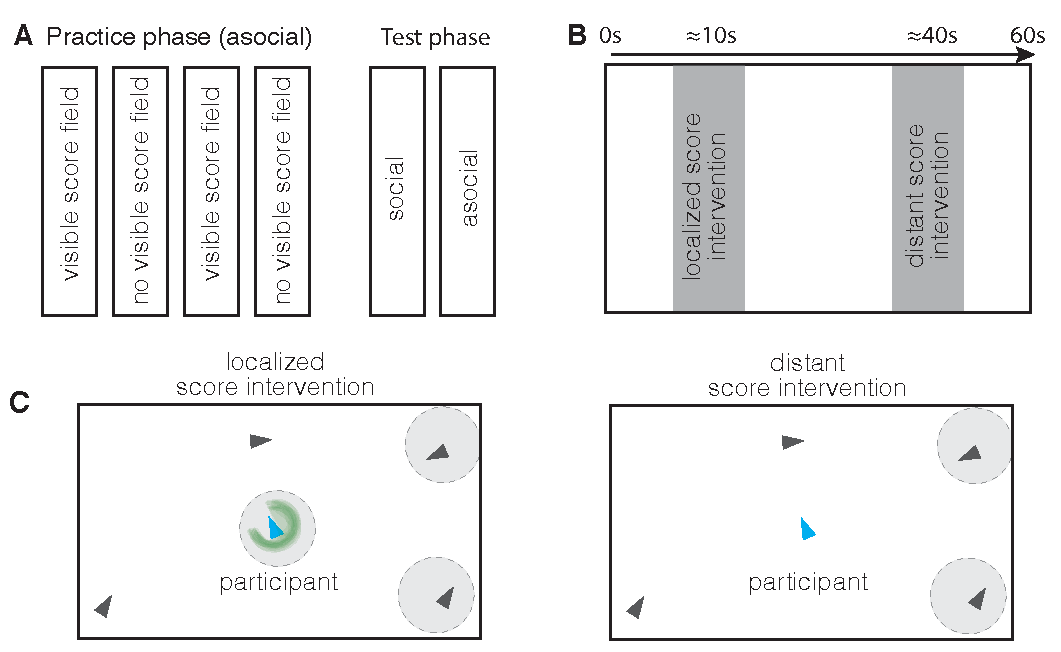
\includegraphics[width=1\textwidth]{./figures/exp2_design.pdf}
  \caption{Design of Experiment 2. (A) The timeline of the test round involves a baseline condition with no score field, and two causal interventions on the score field beginning at approximately 10 seconds and 40 seconds. (B) These interventions manipulate the location of the score field to ensure the player is receiving high reward or not, respectively, while a subset of other agents are receiving high reward.}
  \label{fig:exp2_design}
\end{figure}


\paragraph{Practice phase}

To acclimate participants to the task environment, each game began with four one-minute long practice rounds. 
In the first and third practice rounds, the score field was \emph{visible} to the participant so they could observe its dynamics.
In the second and fourth practice rounds, the score field was invisible to the participants, as in Experiment 1. 
Additionally, we randomized participants into two different groups, who practiced with different score field dynamics. 
In a ``wall-following'' pattern, the high scoring region moved contiguously along the walls of the playing area. 
In a ``random-walk'' pattern, the high scoring region slowly drifted, as in Experiment 1, from one random location to another within the playing region.\footnote{Because we did not observe any differences in participant behavior depending on the score field dynamics observed during the practice phase, we collapsed over this factor in our analyses.}

\paragraph{Test phase}

After the four initial practice rounds, participants played two one-minute test rounds that were the focus of our analyses. 
In one of the two test rounds, no other agents were present (non-social condition), and in the other there were four bots playing with the participant (social condition). 
We randomized the order of social and non-social conditions across participants. 
Each of these rounds was further divided into three conditions, where we causally intervened on the score fields to better test our hypotheses about exploring, copying, and exploiting behavior. 

For the baseline \textit{blank score field} condition, there was no score field. During these times, all the bots were randomly exploring, with two randomly exploring along walls (in association with the wall score field dynamic) and two exploring the center region (associated with the random walk score field dynamic). 
At the ten second mark and the forty second mark in each round, we introduced the two high scoring regions into the game (see Fig.~\ref{fig:exp2_design}B).
In the \textit{distant intervention} condition, we superimposed the wall-following and random-walk score field patterns to create a bi-modal dynamic score field. 
We centered one high scoring region on a wall-following bot and one high scoring region on a bot in the center region. 
In the \textit{localized intervention} condition, however, we centered the high scoring region on the \emph{participant}, wherever they were \andrew{and also on two distant bots (this is what the figure suggests...)}. In this condition, they automatically received a high score for roughly the ten second duration that the high scoring regions were present (see Fig.~\ref{fig:exp2_design}C).
We randomized these two interventions to the two windows across participants.

In the non-social round, we simulated the same bots, so that the distribution of score field positions was the same across the two conditions. (The bots were not responsive to the participants behavior, only to each other.) The bot behavior was programmed according to a selective copying model. These bots explore non-socially when no bots are exploiting, and copy exploiting bots when there are any. The two bots along the wall always stayed along the wall, with any copying bot choosing to copy the wall exploiting wall bot, and the bots exploring in the entire playing region also only paid attention to each other in an analogous way.

% \subsection{Hypotheses}

% \paragraph{Testing social behavior:} We included the non-social trial condition as a control to help us adjust our statistical analysis of behavioral mechanisms to account for behavior that looks social by chance. 

% \paragraph{Testing exploring behavior:}  With the blank score field manipulation we are able to test if participants explored randomly or copied other players when nobody in the game was receiving a high score. 

% \paragraph{Testing copying behavior:}  The targeted score field manipulations allowed us to test whether the participant would preferentially click towards the exploiting bots, and if they had any preference for the bots who were operating on the same score field dynamics the participant had practiced on.

% \paragraph{Testing exploiting behavior:}  The purpose of the localized score field manipulation was to see whether participants would exploit when they receive a high score, regardless of what else was going on in the environment.

\begin{table}[]
\begin{tabular}{r|c|c}
                      & Participant receiving reward & Participant not receiving reward  \\ \hline
Selectively copy  & Eagerness \andrew{FOMO? ;)}                  & \multicolumn{1}{c|}{Selectivity} \\ \hline
Indiscriminately copy &  \multicolumn{2}{c|}{Independence}  \\ \cline{1-3} 
\end{tabular}
\caption{Table of behavioral patterns we use as codes.\andrew{OK, I think I get this now.  Could use a little more explanation... }}
\label{tab:qual_scoring_defs}
\end{table}

\subsection{Results}

To analyze our data from this experiment we use a mixed methods analysis involving both a qualitative coding approach and a quantitative analysis of behavioral traces and click data. 

\subsubsection{Qualitative Coding Results}

\begin{figure}[t!]
    \centering
    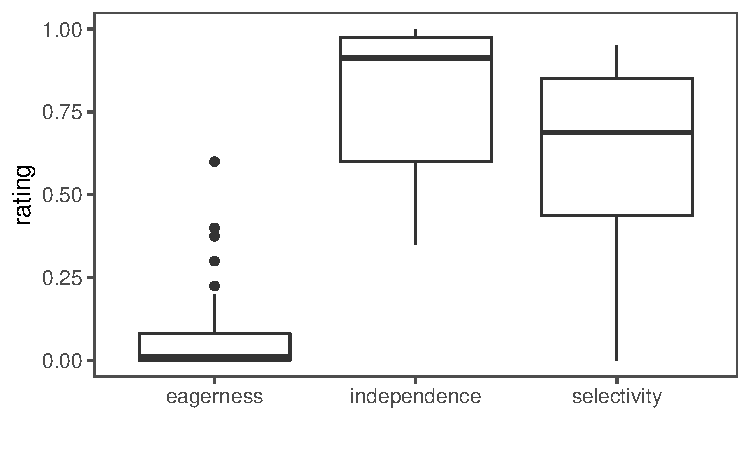
\includegraphics[width=0.9\linewidth]{figures/coding.pdf}
    \caption{Distribution of ratings for three qualitative behavioral properties that were coded from videos. Participants displayed relatively high levels of selective copying behavior and independent exploration, while eager copying is less common.}
    \label{fig:selective}
\end{figure}

For our qualitative analysis, two authors manually coded videos of our 28 participants. We coded for three behavioral signatures --- \emph{selectivity} in copying exploiting bots, \emph{eagerness} in copying other agents, and \emph{independence} in exploration --- on a scale from 0 to 1. \emph{Selectivity} was defined by examining behavior during the combined targeted and non-localized score field manipulations, when the participant was not themselves receiving a reward but another agent was: selectivity was coded as a preference for moving towards agents who were exploiting, as opposed to moving toward agents who were exploring or copying. This behavioral signature marks participants as selectively copying agents who are exploiting the high scoring regions.
\emph{Eagerness} was defined by the same preference for moving toward exploiting agents during the localized score field manipulation event when the participants were always receiving a high score, such that their copying behavior was not contingent on their own state. Eager agents copy even when they could be exploiting the high scoring region they have identify. Eager agents prioritize social information. \andrew{Would be helpful to i) reference Table \ref{tab:qual_scoring_defs} here, and ii) use the terms from that table here (like `indiscriminately copy')}
Finally, \emph{independence} was defined by reverse-coding a preference for moving towards agents who were \emph{not} stopped, at any point in the task. Because we never observed participants copying moving agents when they themselves were already receiving reward, this signature primarily captures whether participants were preferentially moving toward other agents during exploratory periods when there was no evidence of reward in the environment, thus we interpret low prevalence of this signature as high independence. 
The endpoints of the scale roughly represented the proportion of time the participant spent displaying the behavior in question compared to the potentially available opportunities to do so. 

The two coders achieved a correlation of $r = 0.75$ for selectivity, $r = 0.55$ for eagerness, and $r = 0.60$ for independence. The coders resolved disagreements in our codes by averaging. 
First, we found that a substantial fraction of participants display selective copying behavior and independence (Fig. \ref{fig:selective}). 
\todo[inline]{rdh: Is it appropriate to use 0.5 as the null threshold? Do we think that midpoint is meaningful, since even lower numbers, e.g. 0.2, were indicative of some level of these signatures? Maybe should be comparing to a null of 0?}
We found that 71\% of participants had an average selectivity rating of at least 0.5, and 86\% had an average independence rating above that level. 
These proportions were significantly greater than 50\% using a two-sided binomial test, $p = 0.036$ and $p = 0.001$, respectively.  
In comparison, only 1 participant (4\%) was coded as eager at that level, which was significantly less than 50\%, $p < 0.001$.
These qualitative results show that participants appeared to selectively copy stopped agents when they themselves were not receiving reward, but otherwise mostly inhibited social influence.


\subsubsection{Quantitative Behavioral Results}

\begin{figure}
    \centering
    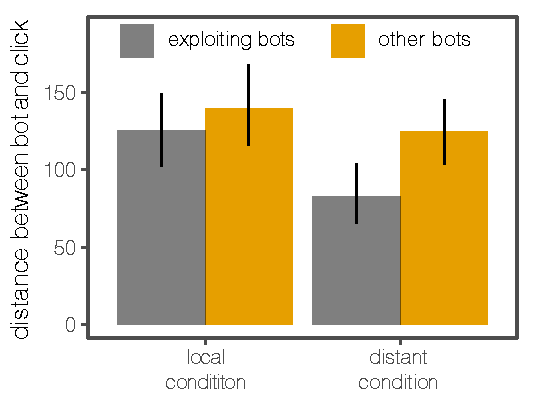
\includegraphics[width=0.8 \linewidth]{figures/proximity.pdf}
    \vspace{-1em}
    \caption{Participants selectively copy agents who appear to be exploiting, but only when they themselves are not receiving reward. Lower pixel distance between bot and click indicates copying. Error bars are bootstrapped 95\% CIs. \todo[inline]{check is nonsocial makes it look better. otherwise relegate to appendix} \andrew{Helpful to define `goal' (is it the click point?). Also, maaaybe better to use something like `focal individual receiving reward', and not, rather than `localized' and distant score condition.  On the other hand, it is nice to use the same terms as in the main text. If I were looking at the figures, without having read the paper, I would not understand these two conditions.}}
    \label{fig:proximity}
\end{figure}

Next, we tested these same hypotheses quantitatively using data we recorded of participants' locations and the state of the environment at each time step of the experiment.
We operationalized copying using participant clicks.
Each click changed their avatar's destination. 
We were interested in the proximity of the new destination to other agents.
To test whether participants selectively to copy exploiting agents, we used information about whether each artificial agent was stopped.
To test whether participants were more likely to copy when they were not already themselves receiving a reward, we compared copying rates across the localized score field condition where the score field was automatically placed on top of the participant and the non-localized, targeted score field condition where it was only placed on top of artificial agents.
We thus constructed a mixed-effects regression model predicting the (minimum) proximity of each click to other agents as a function of condition and whether the other agents were stopped, including participant-level intercepts and main effects (the model did not converge with a random interaction term). 
We found a significant interaction, $b = 51.9, t = 4.5, p < 0.001$, showing a strong selective preference for copying other exploiting agents but only in the condition when the participant was not themselves receiving a reward (see Fig. \ref{fig:proximity}). 
\todo[inline]{rxdh: do we also want to report the significant interaction with the non-social condition here (i.e. that this selectivity was not observed with the `invisible' bots, making it unlikely to observe such a pattern by chance). Otherwise, we're not actually using the non-social condition anywhere in the results.}\andrew{Seems like a good idea. Or just cut the non-social condition from the experimental section, to remove some burden on the reader...}

\section{Experiment 3: Generalizing to more complex environments}

To generalize our understanding of these mechanisms to more complex environments, and to more explicitly compare our findings to the nonhuman animal literature, we conducted a final experiment using the materials designed by \citeA{berdahl_emergent_2013} to examine collective sensing in fish.
These environments are significantly more complex than the binary spotlight and border environments we used in Experiments 1 and 2.
They require agents to use continuous gradients to navigate noisy and fluctuating score fields.
We manipulated the level of noise across different groups, predicting that the cognitive mechanisms discussed in the previous sections may be less reliable under noisier conditions. To test that the social learning strategies identified in the previous experiments also generalize to different external behavioral signatures, we also modified several other aspects of the experiment interface.
For example, a small change in the movement controls led to a different downstream visual cue of success, which flexible agents making social inferences should be able to use for selective copying just as effectively as participants in the previous experiments were able to use the cue of completely stopping.

\subsection{Methods}
\subsubsection{Participants}

We recruited 563 unique participants from Amazon Mechanical Turk to participate in our experiment.
All participants were from the United States.
After excluding 72 participants due to inactivity or latency, and 6 others for disconnecting in the first half of the game, we were left with usable data from 437 participants in 224 groups.
113 individuals (63 groups) were in the low noise condition and 324 individuals (161 groups) were in the high noise condition. 
These groups ranged in size from one to six individuals.  
Since only one group of size six completed the task without disconnections, we ignored this group in our analysis.

\subsubsection{Stimuli and Procedure}

\begin{figure}
  \centering
  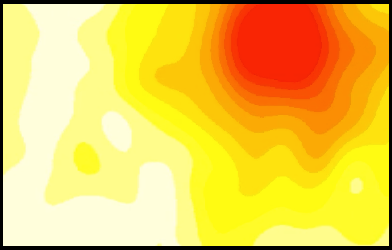
\includegraphics[width=0.4\textwidth]{./figures/easy-field}
  \hspace{0.1cm}
  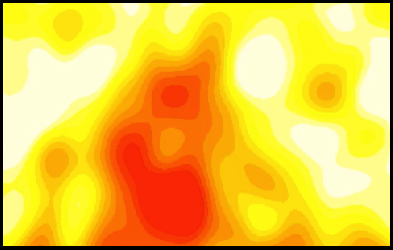
\includegraphics[width=0.4\textwidth]{./figures/medium-field}
  \caption{Example score fields from the low noise (left) and high noise (right) conditions at particular points in time.  Red areas indicate higher scoring areas.}
  \label{fig:score_exp3}
\end{figure}

%Based on the method reported by Berdahl et al., we added 

Our primary change from Experiments 1 and 2 was switching from a binary score field to a more complex, gradient score landscape.
These more complex fields were generated using the method reported by \citeA{berdahl_emergent_2013}. 
We began with the same randomly moving ``spotlight'' of high value as before. 
However, we then combined the spotlight with a field of spatially correlated, temporally varying noise.  
By manipulating the proportional weighting of the noise field and the spotlight, we generated two different conditions, corresponding to two of the noise levels used by \citeauthor{berdahl_emergent_2013}. 
In the \emph{low noise} condition, the spotlight was weighted strongly compared to the noise field (10\% noise), with the noise field providing minor background variation (see Fig. \ref{fig:score_exp3}, left). 
In the \emph{high noise} condition, the weighting of the noise field was increased (25\% noise), providing more extreme fluctuation outside of the spotlight (see Fig. \ref{fig:score_exp3}, right).
To decrease variability and increase statistical power, we generated only four distinct score fields per noise level, so multiple groups experienced the same fields.  

In addition to these more complex score fields, we made several adjustments to the interface.
First, rather than showing their current score as binary---a glowing halo around the player when inside the spotlight---their score was presented as a percentage at the top of the playing area (see Supplemental Fig.~\ref{fig:exp3_interface} for a screenshot).
Second, rather than clicking to change direction, players controlled their avatars using their keyboard. 
The left and right arrow keys were used to turn (at a rate of $40^\circ$ per second) and the
spacebar was used to accelerate. 
Unlike before, we did not provide a mechanism to stop completely.  
Given the closer relation to \citeA{berdahl_emergent_2013} in this experiment, it is also relevant that the speeds of the avatars and the playing area dimensions ($480 \times 285$) throughout all of our experiments were matched to those reported by Berdahl et al.; in this experiment, we additionally used the same total task length of six minutes.

The procedure was similar to Experiment 1: after successfully completing a comprehension test,  participants were redirected to a waiting room where they could get used to the controls.  
Participants were not given any practice rounds, or any information about the nature of the underlying score fields.
The conditions for removal due to inactivity or latency, and the bonusing scheme, were also similar to Experiment 1 with slightly different parameters.

\begin{figure}[t]
  \centering
  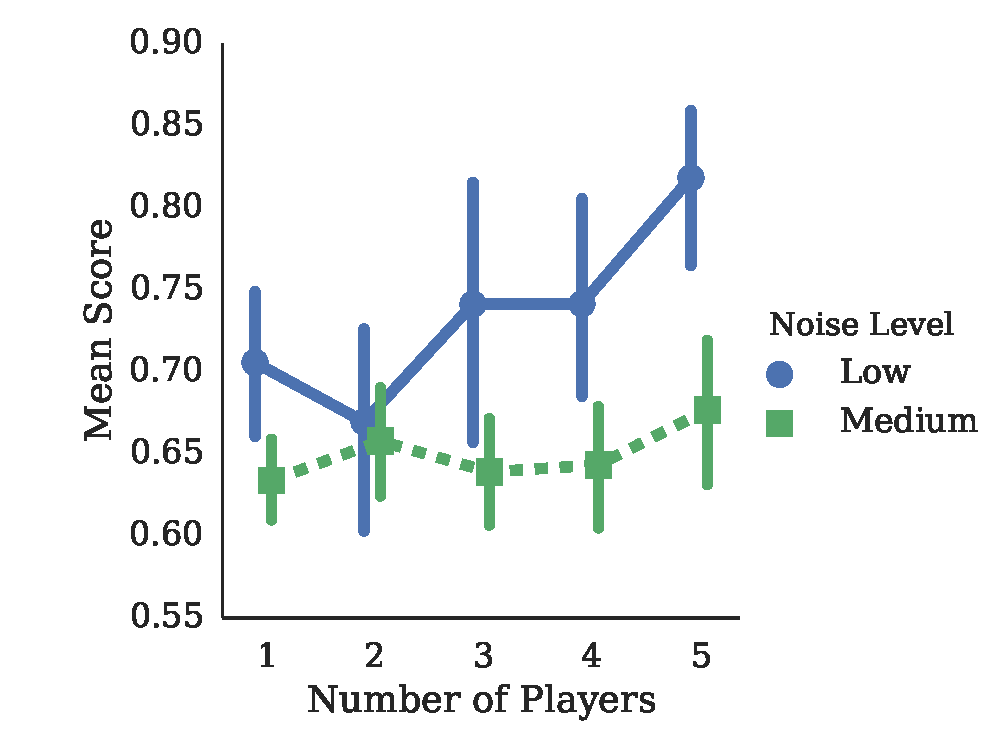
\includegraphics[width=0.8\textwidth]{./figures/performance-summary}
  \caption{Mean performance as a function of group size in the low and
    medium noise levels.  Error bars are 95\% bootstrap confidence
    intervals using the group as the primary bootstrap unit.  All
    points are averages over at least two groups.  This plot excludes
    the single group we were able to collect of size six.  Including
    this group weakens the trend in the medium noise condition. \andrew{Do we want to `normalize' the scores, for example, by seeing what performance they would get against 100 random score fields they did not experience, so that the reader has a sense of how much better than expected these performances are?}}
  \label{fig:performance}
\end{figure}

\subsection{Results}

Our analyses focus on two primary questions: (1) how does the introduction of a noisier environment affect collective performance, and (2) how do the selective social learning strategies identified in Experiment 2 play out in such an environment, when inferences about the success of other agents may be less reliable?

\subsubsection{Effects of noise on collective performance}

We begin by analyzing patterns of collective performance across groups of different sizes and across the different noise conditions.
As our measure of performance, we computed the average score obtained by participants over the second half of the experiment.
To test effects of performance, we constructed a mixed-effects regression model.
We also included random effects for each group (i.e. controlling for possible correlations between participants in the same group) and for each score field (i.e. controlling for the possibility that some randomly generated score fields were more difficult than others).

\todo[inline]{TODO: put in numbers.}
We found a significant interaction between group size and noise condition ($b = $). 
As in Experiment 1, performance in the low noise condition increased significantly in larger groups.  
However, there was less improvement with larger group size in the high noise condition (see \ref{fig:performance}). 
Examining the simple effects of group size at each noise level reveals a significant effect of group size for the low noise condition ($b = $), and no significant effect for the high noise condition ($b = $). 
Moreover, examining the random effects also revealed larger variability due to score field in the ``high'' noise condition than the ``low'' noise condition.
One particular score field in the high condition displayed a significant effect of group size, while none of the others do. 
Qualitative inspection revealed that this particular score field seemed to share spatial properties more similar to the low noise score fields (e.g. fewer local maxima).  
\todo[inline]{Double-check this?}
Overall these results indicate an important role of the environment in group success: under low noise, larger groups perform systemically better on our task than smaller groups, similar to the effect found in Experiment 1, yet no such benefit is found under higher noise conditions.
\andrew{Do you think this is due to mini `reward zones' being small and ephemeral, (rather than just the big blob), so that even if you copy, by the time you get over there, it is gone? Duration of spin events vs noise? Distance of spin even from center of blob?}
%The improvement we found in the low-noise condition contrasts with the lack of any improvement found by \citeA{berdahl_emergent_2013} in fish groups at the same sizes.
%The effect of noise also contrasts with the apparent invariance to noise conditions found in fish behavior.

\subsubsection{Analysis of social learning strategies}

Next, in order to understand the mechanisms that may have contributed to these effects of noise on collective performance, we more closely analyzed the behavior of the players in our games.
Unlike in Experiment 2, where click data provided a useful measure of copying, we approached this analysis with a simple state-based representation of player behavior based on their keyboard movements.
We empirically determine the state of each player at each point in time --- exploring, exploiting, or copying --- using a simple set of hand-specified criteria.
All of these criteria depend only on information that is observable to any player in the game (i.e., the filters do not depend directly on the scores of any individuals), and hence we can use these states as proxies for what other players might infer.
Also, since the states are not defined in terms of scores, we can meaningfully quantify the relationship between state and performance.

Our criteria for classifying the three states are as follows.
\begin{itemize}
\item \emph{Exploiting} behavior was not trivial for players since the avatars always move at least at a slow constant velocity. 
Unlike in the previous experiments, where the ``s'' could could be pressed to stop in place, a player in Experiment 3 could either meander around a particular location or persistently hold down one of the arrow keys while moving at a slow speed, which creates a relatively tight circular motion around a particular location.  
We call this second activity ``spinning'' because of its distinctive appearance.  
We then classify a player as exploiting if the player is spinning for 1 second, or if the player moves at a slow speed for 3 seconds and has not traveled more than two thirds of the possible distance that the player could have traveled in that time.
The second condition is captures the meandering behavior of individuals who have not discovered how to spin. \andrew{Is there evidence that any players learned to spin from others? That would be a cute side story: social learning of a mechanism that leads to emergent collective sensing} 
\item \emph{Copying} behavior is more difficult to identify, but is likely characterized by directed movements towards other players. 
We thus classify a player as copying if they move at the fast speed in a straight line towards any particular other player for a 500ms window.
We consider a player to be moving towards another player if the second player is within a $60^\circ$ on either side of the first player's straight-line trajectory.
\item We classify behavior as \emph{exploring} if the player is neither exploiting nor copying. Thus, a player will be classified as exploring if that player is either moving slowly but not staying in the same general location, if the player is moving quickly but not towards any particular person, or if the player is moving quickly and turning.
\end{itemize}

\begin{figure}[t!]
  \centering
  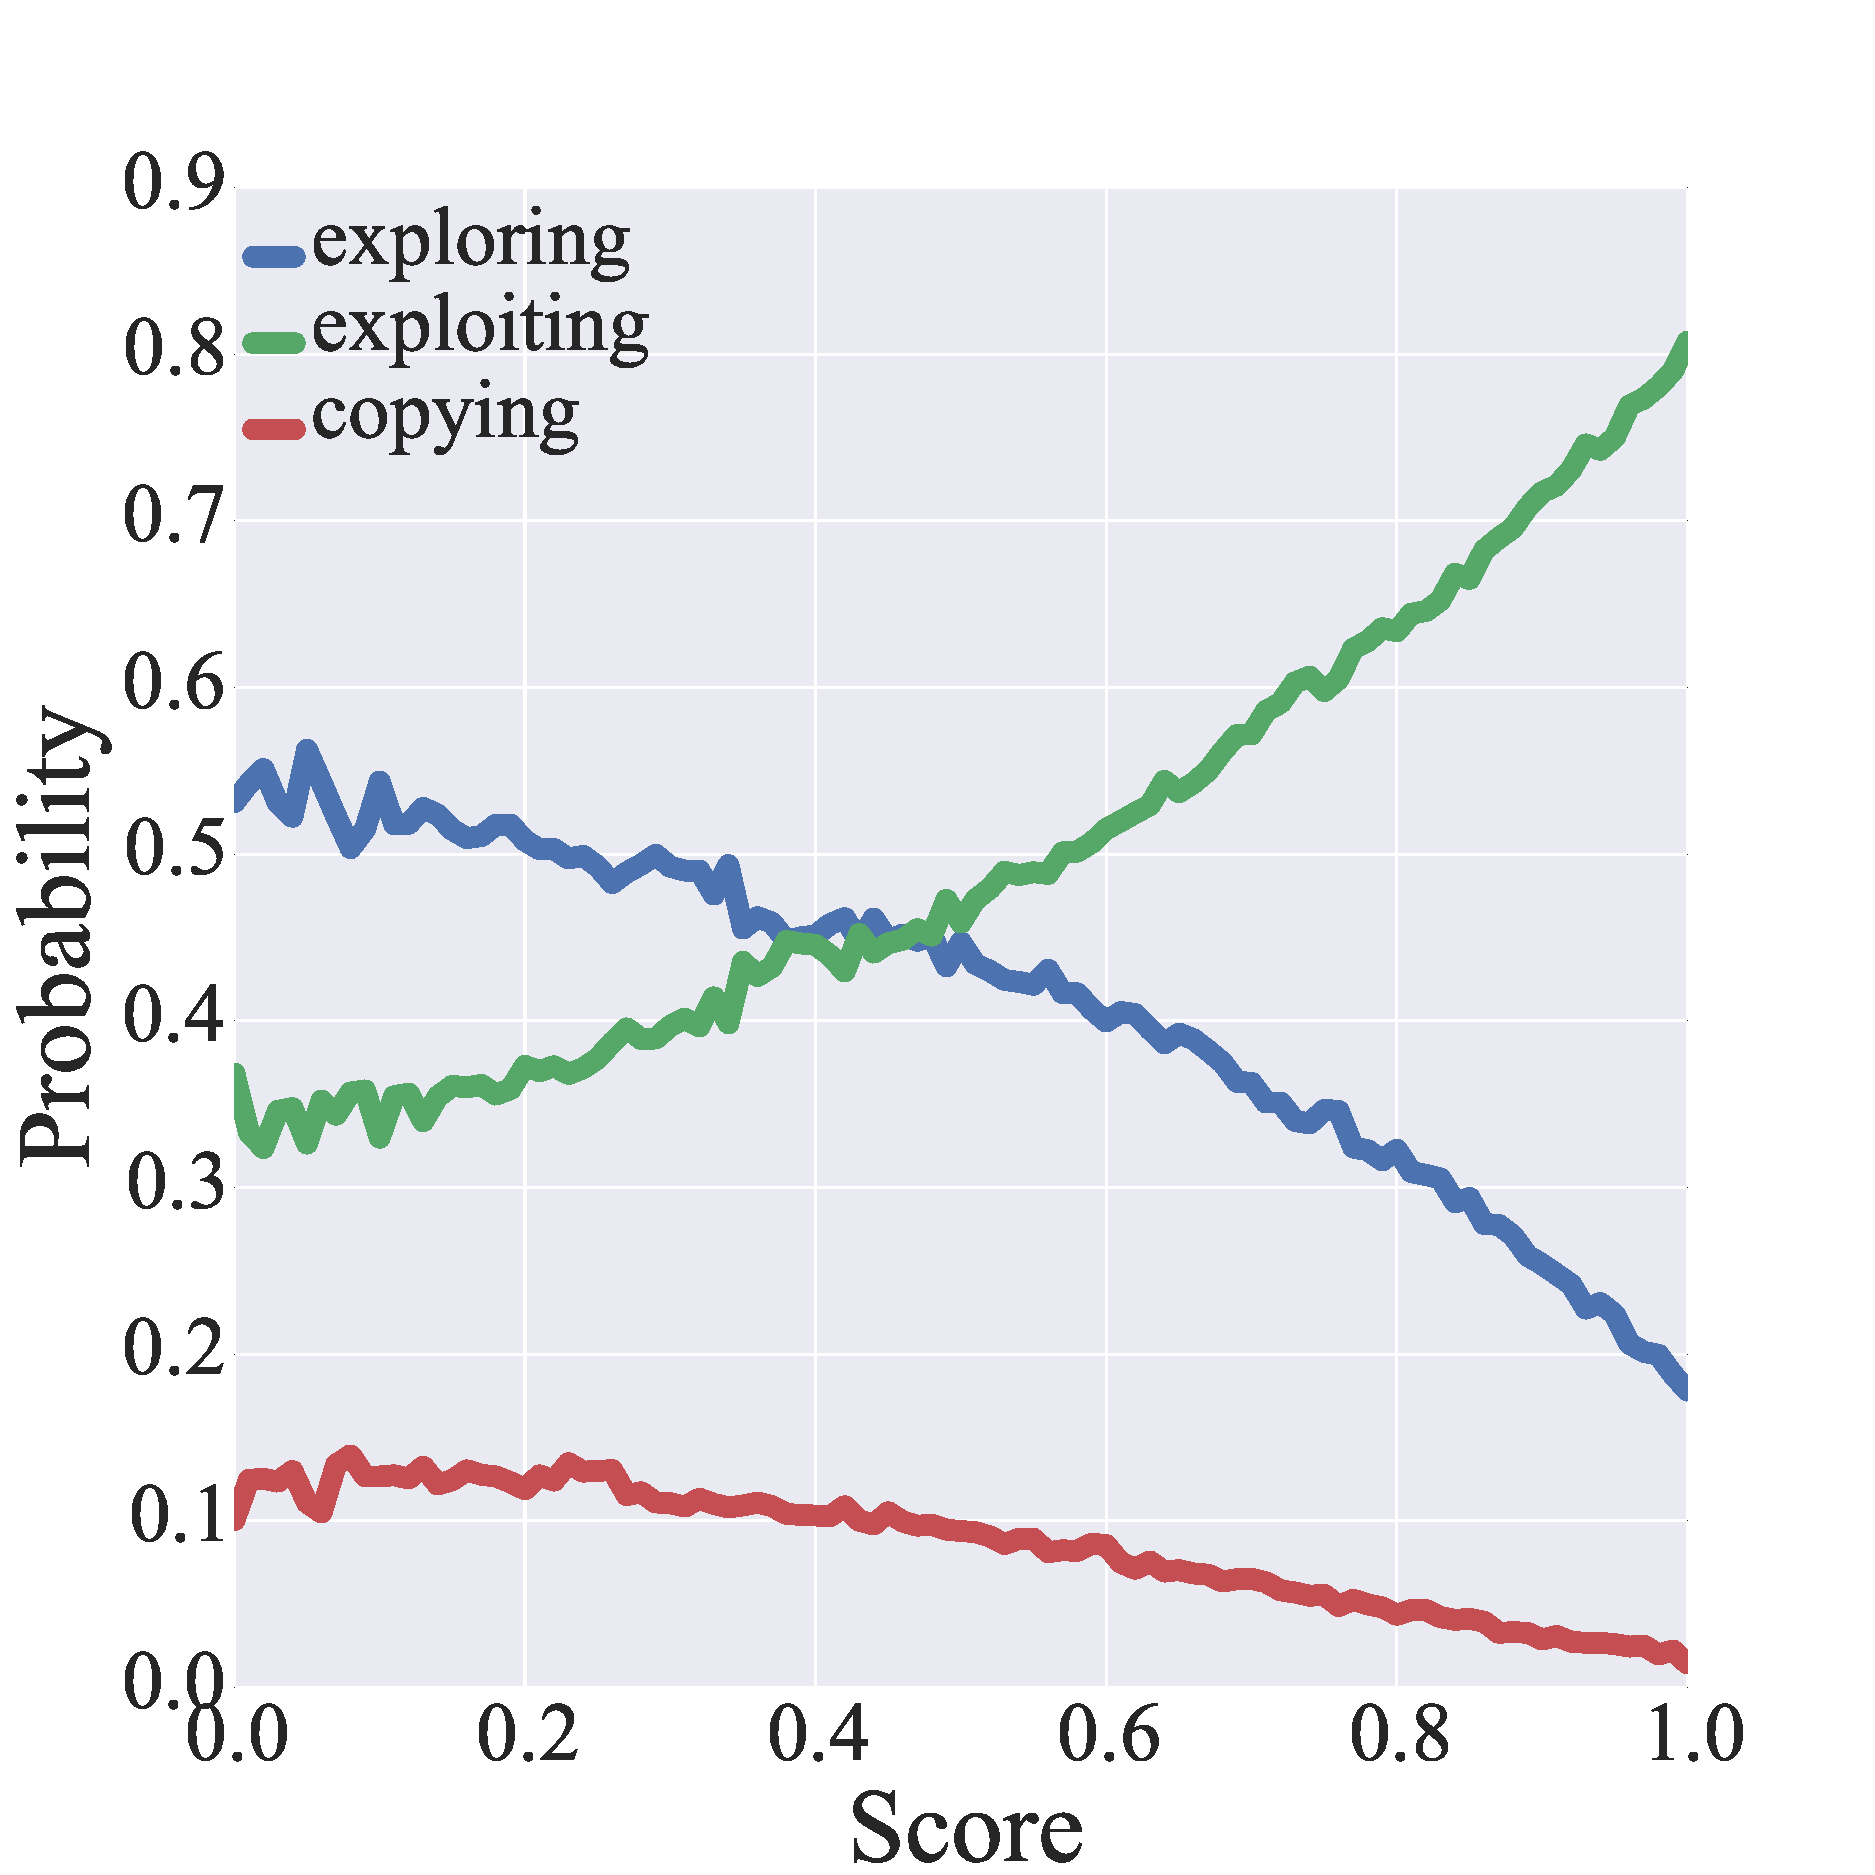
\includegraphics[width=0.8\textwidth]{./figures/states}
  \caption{The probability of an individual being in a particular
    behavioral state as a function of the individual's score. \andrew{Is this for both noises combined?  If they are separated, do we see copying is stronger in the low noise treatment?}}
  \label{fig:states}
\end{figure}

\todo[inline]{rxdh: first, let's report a multinomial regression here on the state proportions? And show a plot where the low \& high noise, and all groups sizes are collapsed together as first panel of Fig.?}
We now proceed to use this classification scheme to analyze the behavioral strategies used by participants in our game.
First, in line with our finding in Experiment 2 that participants inhibit copying when they find themselves in high-scoring regions, we predicted that the probability of the exploiting state would increase as players receive higher scores.  
To test this prediction, we constructed a multinomial mixed-effects regression model predicting the probability that each individual is in each of the three states at each point in the game. 
We included fixed effects of current background score, noise condition, and group size, as well as random intercepts for each group and background field.
We found that the probability of a player occupying a particular state is closely related to that player's score (see Fig.~\ref{fig:states}A). 
Specifically, players are significantly more likely to be in the exploiting state in higher scoring locations than in lower scoring locations ($b=$, $p=$).
This selectivity in exploiting behavior has the adaptive property that players will tend to remain in good areas and will leave bad areas quickly either by exploring independently or by copying other individuals.


\todo[inline]{rxdh: look at duration of spins, and distance of spin from the blob center?}


\todo[inline]{rxdh: second, let's break it out by noise and group size for second panel of Fig., and analyze how environmental noise conditions may affect strategies, suggest this may help explain gaps in scores?}\andrew{Yup! Great idea.}
Second, we examine how the deployment of these behavioral states may vary with higher or lower noise in the environment. 
In the same regression model, we examine the effect of noise condition and find that participants are significantly more likely to be exploiting in the high noise condition, even at lower values ($b=, p=$; see Fig.~\ref{fig:states}B), and thus less likely to be copying or exploring overall.
A lower threshold for exploiting may help explain the gaps in collective performance across noise conditions, as it also makes copying less effective: the external signatures of exploiting (e.g. ``spinning'' behavior) are less strong evidence for inferences of success. \andrew{yes cool, so in the high noise, there might be less tendency to copy, but also less opportunity to copy due to less spinning.  Wait, can we get at the less tendency to copy, independent of the reduced opportunity?}

\todo[inline]{rxdh: third, we can zoom into properties of copying behavior more specifically, and revise this paragraph with the updated results (e.g. we took out the correlations of higher performance with better copying; do we want to replace it with something more specifically related to Exp. 2? Like showing the *targets* of copying tend to be in higher scoring regions?)}
Third, while our previous analyses focused primarily on the exploiting state, we now turn to analyzing the properties of copying. 
In Experiment 2, we found that participants did not copy indiscriminately but were able to selectively copy players receiving high rewards, even though these rewards were not directly visible. 
In this experiment, we likewise examined the scores of the players who are being copied.
\textbf{Result here...}
Moreover, as shown in Figure \ref{fig:proportion}, groups that contain individuals who focus their copying behavior on higher scoring individuals achieve significantly higher performance in our task (slope: 0.2639, 95\% CI: $[0.145,  0.383]$). 
A player who is able to accurately infer whether another player is receiving a high score may be able to achieve higher performance on our task by leveraging these inferences to more effectively copy others.

\section{Discussion}

\todo[inline]{rxdh: need to revise this summary to state the problem again and say briefly the contribution of each experiment.}
Our experiments established that people display collective intelligence in a multi-agent tracking paradigm inspired by experiments conducted with fish by previous researchers, and that people display emergent collective intelligence at much smaller group sizes in our environments than fish do in the setup of prior research. \andrew{Should we mention that the underlying mechanism seems to be quite different...}  In our analyses of Experiments 2 and 3, we also confirmed selective social learning strategies allowing people to achieve collective intelligence in this environment.

\paragraph{Social inference mechanisms in non-human animals.}

\todo[inline]{Can Andrew help extend this?}
\todo[inline]{Notes: seems like both do collective sensing, but mechanisms different. Have advantages and disadvantages. Human algorithm gives good ...}

While we focused on the consequences of fast social inferences in human groups, the status of similar mechanisms in non-human animals remains more controversial.
At least some species, such as cliff-dwelling swallows, appear to engage in signalling behavior at food sites \cite{brown1988social,brown1991food}, which effectively externalizes success and draws conspecifics to enhance the efficiency of foraging \cite{torney2011signalling}.
Many additional cues of success are available as simple by-products of foraging, such as the sound of eating or (more directly) the scent of food \cite{galef2001social}.
However, copying based on these cues may be explained by associative learning or other simple biases.

\paragraph{Comparison to Berdahl et al. (2013).}

Our study design was inspired by collective sensing tasks used in the animal behavior literature, particularly the one proposed for groups of fish by \citeA{berdahl_emergent_2013}. 
We found similar improvements in performance as a function of group size in humans, suggesting that the general phenomenon of collective intelligence persists across different species.
At the same time, we observed some key differences, suggesting that these collective intelligence phenomena may arise from different mechanisms.
First, we found that humans were able to achieve increases in performance at much smaller group sizes than fish. 
Fish exhibited mild improvements in average performance at groups of 16 and more substantial improvements at groups of 64 and 128.  
However, we see significant improvements in human performance at just five players. 
Second, while there was no difference in the effect of group size across different environmental noise levels for fish, we found that in the small-group regime we considered, the benefits of larger group sizes only accrued in low-noise conditions for humans.

%This difference in the small-group regime may be at least partially explained by the differences in the mechanism that humans appear to use in this task as compared to fish.

% Golden shiners prefers to spend time in dark areas of the water, presumably to avoid predators.  
% In this task, the researchers studied the effectiveness of the fish at finding the darker areas of the tank as a function of the number of fish participating in the task.  
% The researchers found that average group performance increased significantly as a function of group size, and they identified two simple behavioral mechanisms driving this improvement:
% First, individual fish tended to move more slowly in darker areas. 
% Second, individual fish also tended to turn towards conspecifics.  
% This experiment provides a striking example of a higher level of intelligence at the group level emerging from minimal intelligence at the individual level.

These differences may partially be explained by the different mechanisms identified in our different studies.
\citeA{berdahl_emergent_2013} explains collective sensing in fish as an emergent consequence of two more general-purpose processes: (1) the modulation of speed in preferred regions and (2) the general, un-targeted tendency to orient toward other agents.
These mechanisms have both similarities and differences with the social inference mechanisms we have identified in humans.
Similar to our finding in Experiment 3 that humans modulate their exploring vs. exploiting behavior based on their current score, fish modulated their speeds based on the level of darkness that they were experiencing.  
Fish moved slower in their preferred darker areas and faster in lighter areas.  
And, similar to the copying behavior we observe, fish had a tendency for turning towards other fish.  
However, the model of fish behavior  did not require any social inference or selectivity. 
Whereas fish appear to equally weight all nearby conspecifics, humans modulate their copying behavior based on the inferred scores of other players.
Additionally, we found that humans strategically deploy \emph{independent} exploration (i.e. explicitly ignoring or moving away from all other agents at times) rather than constantly being pulled toward the locations of other players. 
These differences support recent work in social learning \cite{wisdom_social_2013, mcelreath_beyond_2008}, which find flexibility in the strategic deployment of imitation in humans.
It remains difficult to make broad comparisons of human performance to the performance of fish given the differences between the perceptual and motor abilities of fish in an tank and those available to participants in our simulated environment. 
Yet our study nonetheless raises interesting potential differences in mechanism.  

\paragraph{Organizational behavior.}

\todo[inline]{Maybe tie these together with a transition about connections to human?}

Beyond the recent literature on collective intelligence in nonhuman animal groups, there has been a long line of work studying the factors that predict the performance of human groups in various scenarios \cite{kerr_group_2004}.  
Our findings are consistent with previous work suggesting that having a larger group is beneficial in complex, uncertain environments \cite{stewart_meta-analytic_2006}.  
Unlike much of this previous work, however, we focus here on the possibility in larger groups of new emergent group abilities and behaviors, and on the mechanisms leading to these emergent properties.

\paragraph{Metacognitive Reasoning.}

People in our experiments displayed remarkable ability to adapt to the new environment they entered for these experiments. For fish, the ability to
gain from group performance in these collective sensing tasks is
likely based on innate behaviors, selected over many generations of
fish facing exactly this problem over their whole lifespans.  In
contrast, some of our humans groups, facing this particular problem
for the first time, appear to have discovered reasonable collective
sensing strategies in just a matter of minutes.

%Nevertheless, our comparison hints at a superior capacity for distributed cognition in humans, possibly enabled by our ability for theory of mind.

\paragraph{Contextual Factors.}

The picture of collective intelligence in humans and across specifies that is emerging from the scientific literature is that different mechanisms give rise to collective intelligence in different species, and that certainly the same can be said even of the different types of human collective intelligence displayed in different contexts.  Human collective intelligence on Wikipedia operates in a way that is very different from human collective intelligence (or unintelligence) on social media platforms like Twitter, and both are quite different from the mechanisms of collective intelligence through which bees find new homes or ants scavenge for food. 

The mechanisms we identify in our experiment are yet another context.

Still, the quest continues for what general abilities and principles underlie the range of intricate and sophisticated forms of human collective intelligence, and distinguish those as a group from the apparently simpler, more swarm-like forms of collective intelligence found in species such as social insects or fish.  Focusing on cognitive mechanisms rather than general strategies may provide a more domain-general way to understand collective intelligence.

\paragraph{Conclusions.}
\todo[inline]{rxdh: this needs to be lightly revised to make sure it flows with rest of argument (currently verbatim from cogsci paper). e.g. the observation about collective memory of actions might be better suited in a previous discussion paragraph?}
\todo[inline]{pk: scrap if we can't think of something better?}
Our work sheds light on one of the pressing puzzles of
human collective intelligence and human distributed cognition.  What
are the abilities that underlie specific mechanisms by which humans establish effective
coordinated distributed information processing agents that can
accomplish more than any individual alone?  The perspective of group behavior as
distributed processing \cite{hutchins_cognition_1995} suggests the
importance of communication for collective intelligence because of the
importance of communication in distributed systems.  
%Moreover, theory of mind---an enabler of implicit communication---has been shown to be predictive of collective intelligence \cite{woolleyevidence2010,  engelreading2014}.  
Our work further
suggests that one of the roles that theory of mind plays in the
emergence of collective intelligence is facilitating implicit
communication that allows for coordination on good collective actions.
Moreover, our work also suggests that the benefit of a group's
coordinating on good actions could be more than simply the benefit to
each individual independently.  By combining a natural human tendency
for independent exploration with a discerning social awareness, humans
appear to be able to fluctuate between exploiting known good actions,
independently exploring new options, and intelligently copying the
promising choices of other individuals.  A simultaneous combination of
these activities by a cohesive group appears to lead to a collective
memory of recently good actions from individuals who continue to
exploit, and a collective movement towards actions that promise to be
good in the near future driven by independently exploring individuals.
The reactive distributed sensing ability that appears to emerge from
this process may confer a unique benefit to working together in
tightly knit groups.
%%who either find new good areas or return to the group.
%% The exploiting
%% core form the body of the group and the exploring individuals form the
%% sticky appendages that drive the group's gradual crawl.

\section{Acknowledgments}

\small

This material is based upon work supported by the National Science
Foundation Graduate Research Fellowship under Grant No. 1122374 to PK
and Grant No. DGE-114747 to RXDH. Any opinion, findings, and
conclusions or recommendations expressed in this material are those of
the authors(s) and do not necessarily reflect the views of the
National Science Foundation.  This material is based upon work
supported by the Center for Minds, Brains and Machines (CBMM), funded
by NSF STC award CCF-1231216.
\andrew{Can we thank Torney for providing the code to make the score field gradients?}


\bibliographystyle{apacite}

\setlength{\bibleftmargin}{.125in}
\setlength{\bibindent}{-\bibleftmargin}

\small{
  \bibliography{couzin}
}


\section*{Appendix A: Behavioral Model}

The trends we observe suggest a potential set of behavioral mechanisms
that effective human groups may use in our task.  We propose that each
player in an effective group chooses a state based on the following
rules:
\begin{enumerate}
\item
  If the player is in a good area, the player will remain in that area
  exploiting.
\item
  If the player in not in a good area and the player perceives another
  person as possibly having a higher score, the player may choose to
  copy that person.
\item
  Otherwise the player will explore independently.
\end{enumerate}

According to this model, players in bad locations improve their scores
by copying exploiting individuals instead of wasting time by copying
low scoring players or wasting time by exploring many poor quality
areas.  The model also has interesting emergent collective properties.
When any individual finds a good area, that player will attract the
other players to that location by exploiting.  Then, when all the
players are together in a group exploiting a particular area, one of
the players will start to lose bonus as the score field shifts.  This
player will then either move closer to the others who are still
exploiting or will shift to an exploring state.  If that player starts
exploring but doesn't find any good locations, the player will return
to the group if the group is still exploiting.  If that player does
find a new good area, though, the player will start exploiting that
area.  The rest of the group will then follow after the highest
scoring region shifts to where the exploiting player is.  This
mechanism creates a kind of gradual crawling that effectively tracks
the moving score field.  Thus, by using this mechanism players are
improving both their own performances directly and also that of the
entire group by participating in this process of emergent collective
sensing.  An example of this process occurring in participant gameplay
is shown in Figure \ref{fig:example}.

\begin{figure*}
  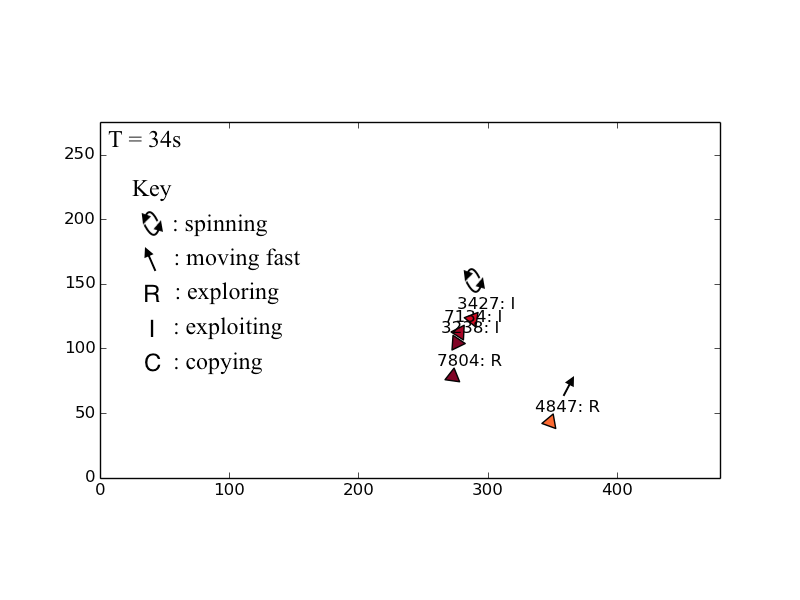
\includegraphics[width=0.33\textwidth,trim=2.5cm 3cm 2cm 3cm,clip]{./figures/pos0274}
  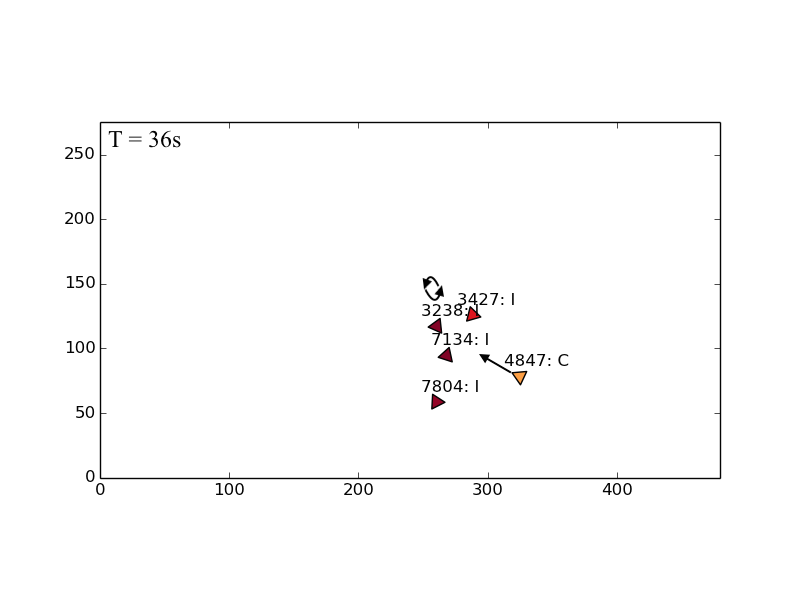
\includegraphics[width=0.33\textwidth,trim=2.5cm 3cm 2cm 3cm,clip]{./figures/pos0285}
  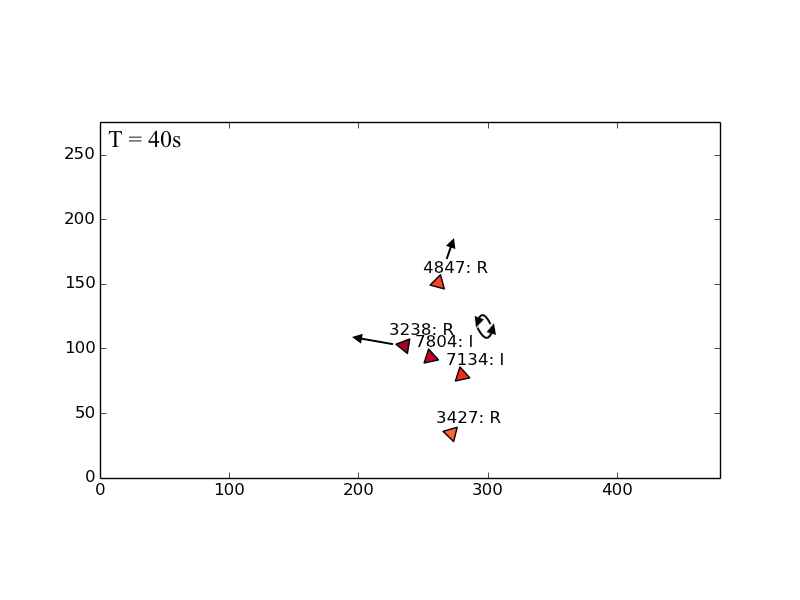
\includegraphics[width=0.33\textwidth,trim=2.5cm 3cm 2cm 3cm,clip]{./figures/pos0323}\\
  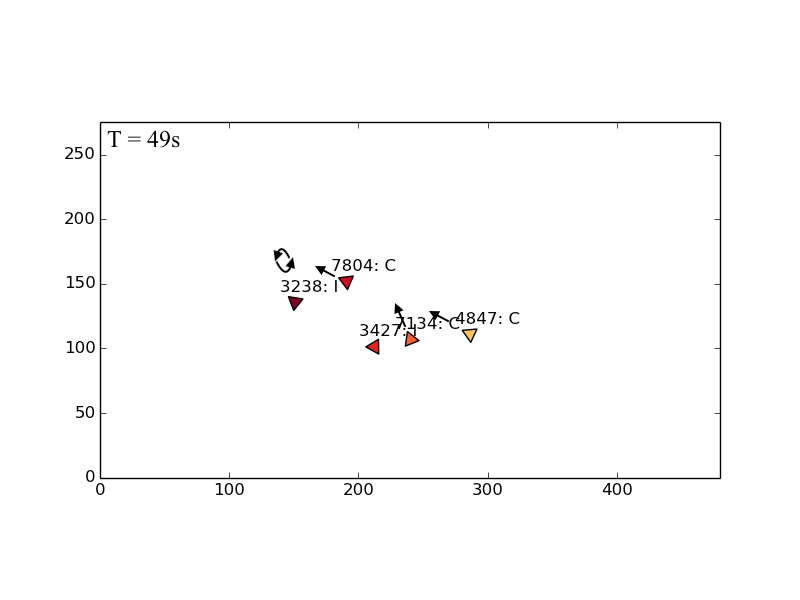
\includegraphics[width=0.33\textwidth,trim=2.5cm 3cm 2cm 3cm,clip]{./figures/pos0394} % 388
  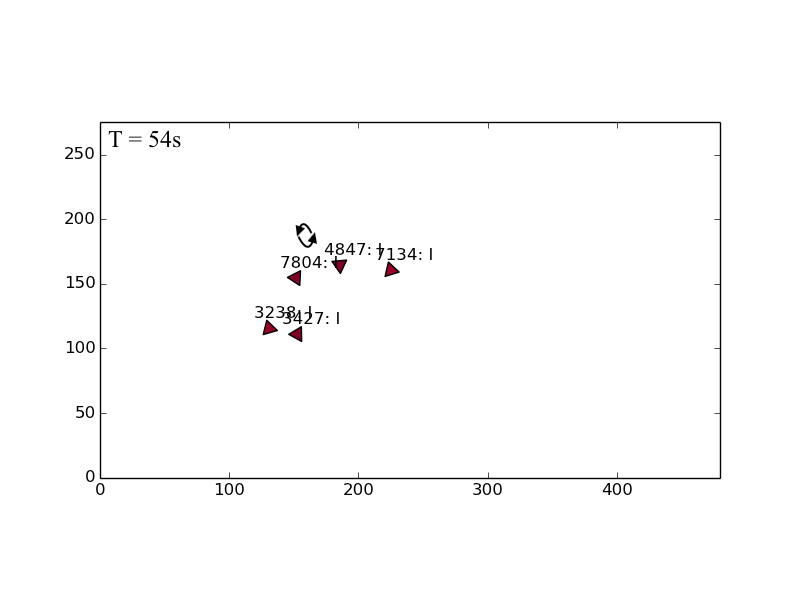
\includegraphics[width=0.33\textwidth,trim=2.5cm 3cm 2cm 3cm,clip]{./figures/pos0435}
  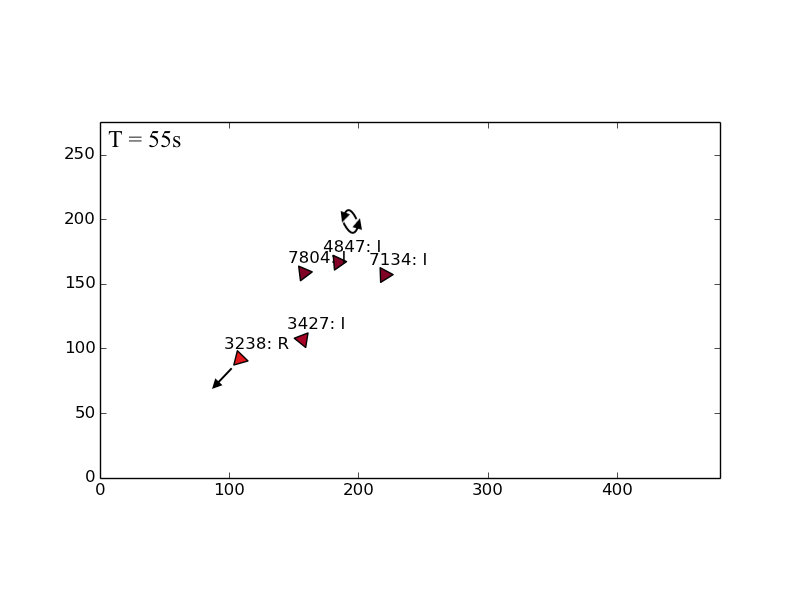
\includegraphics[width=0.33\textwidth,trim=2.5cm 3cm 2cm 3cm,clip]{./figures/pos0441}
  \caption{Reconstructions of actual gameplay in a five-person group
    illustrating both failed exploration leading to intelligent
    copying and successful exploration leading to collective
    movement. Colors indicate the individuals' scores, with red being
    higher and orange/yellow being lower.  The player labels indicate
    both player IDs and also the player states our feature extraction
    procedure inferred.  Other annotations are provided to give a
    sense for the game dynamics.  At $34$ seconds, in the first panel,
    most of the group has converged on exploiting a particular area
    while one individual is exploring independently.  To the right, at
    36 seconds, the exploring individual appears to have failed to
    find a good location and ceases exploring by copying the group.
    At 40 seconds, the final panel in the first row, the score field
    has shifted and some of the group begins exploring while others
    continue to exploit.  By 49 seconds, the first panel in the second
    row, one of the exploring individuals found a good location, and
    other players have begun to move towards that individual.  At 54
    seconds, the entire group is exploiting the new area.  In the
    final panel, at 55 seconds, the background has shifted enough
    again that one of the individuals begins to explore.}
  \label{fig:example}
\end{figure*}


\begin{figure}
  \centering
  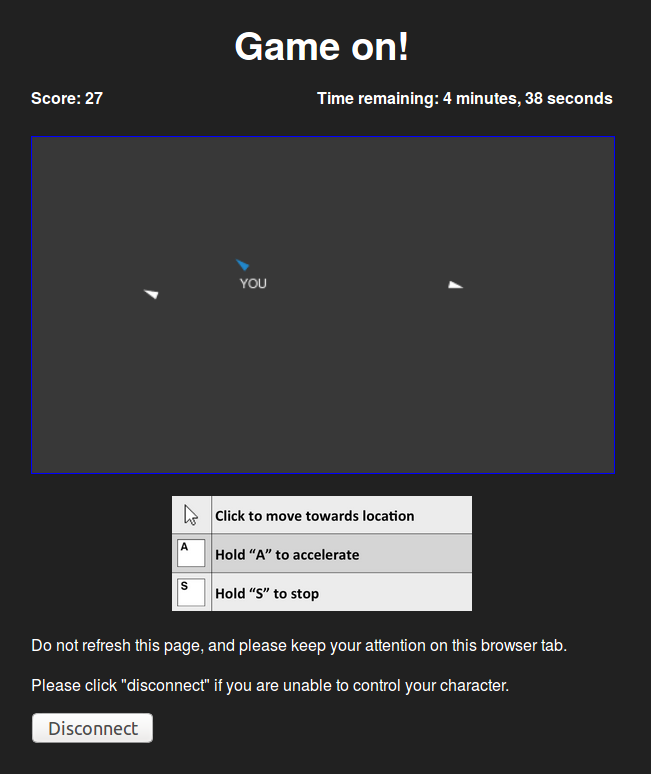
\includegraphics[width=0.3\textwidth]{./figures/experiment-3-no-score}
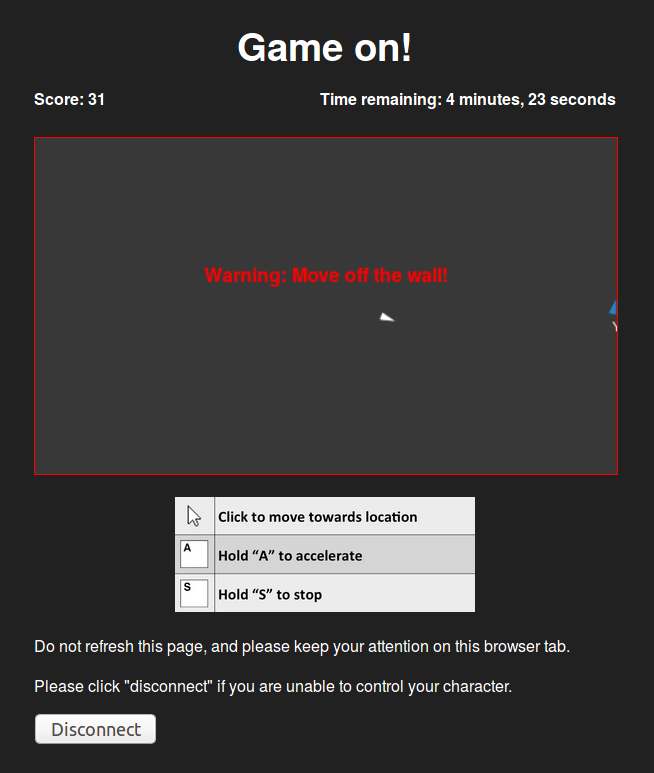
\includegraphics[width=0.3\textwidth]{./figures/experiment-3-wall}
  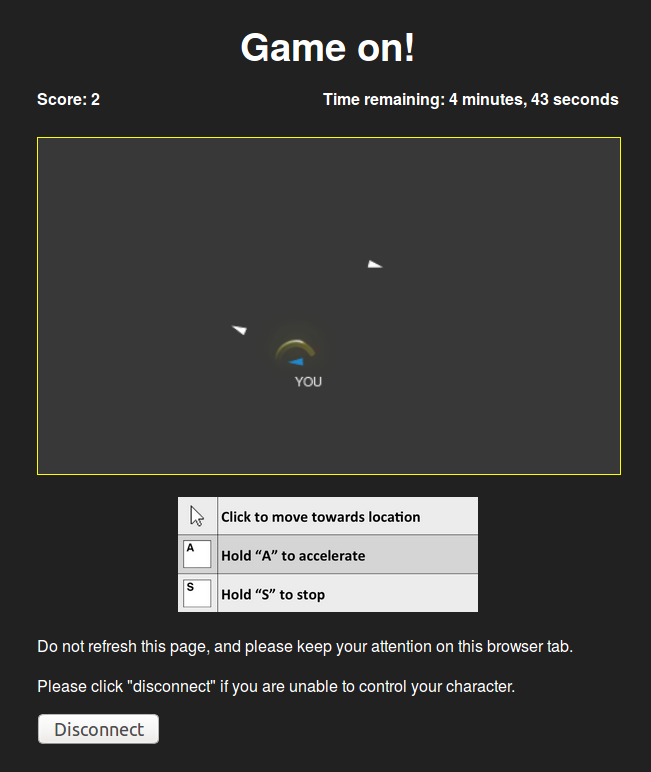
\includegraphics[width=0.3\textwidth]{./figures/experiment-3-score}
  \hspace{0.1cm}
  \caption{Examples of Experiment 1 interface.}
  \label{fig:supplemental_interface}
\end{figure}


\begin{figure}
  \centering
  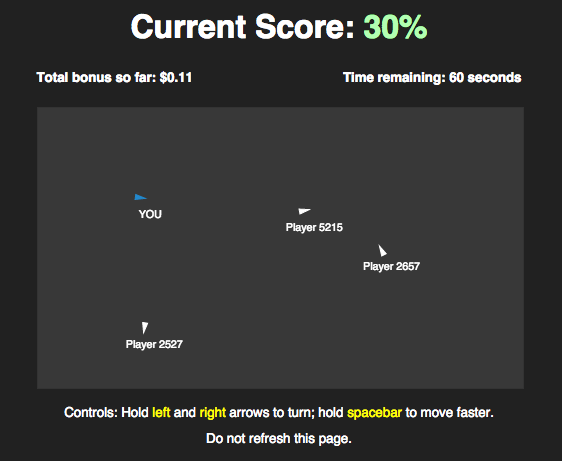
\includegraphics[width=0.9\textwidth]{./figures/interface}
  \caption{Screenshots of the Experiment 3 interface.  The
    score displayed corresponds to the value of the score field at the
    location that the player's avatar is occupying.}
  \label{fig:exp3_interface}
\end{figure}

\end{document}
